\documentclass{article}
\usepackage{graphicx,lineno,fullpage,natbib}
%\linespread{1.5}
\title{Thermal history modelling: {\tt HeFTy} vs. {\tt QTQt}}
\author{Pieter Vermeesch$^*$ and Yuntao Tian \\~\\ 
London Geochronology Centre\\{\it Department of Earth Sciences}\\ 
University College London}
\date{}
\begin{document}

\maketitle

%\linenumbers

\begin{abstract}
{\tt HeFTy} is a popular thermal history modelling program which is
named after a brand of trash bags as a reminder of the `garbage in,
garbage out' principle.  {\tt QTQt} is an alternative program whose
name refers to its ability to extract visually appealing (`cute')
time-temperature paths from complex thermochronological datasets.
This paper compares and contrasts the two programs and aims to explain
the algorithmic underpinnings of these `black boxes' with some simple
examples.  Both codes consist of `forward' and `inverse' modelling
functionalities.  The `forward model' allows the user to predict the
expected data distribution for any given thermal history. The `inverse
model' finds the thermal history that best matches some input
data. {\tt HeFTy} and {\tt QTQt} are based on the same physical
principles and their forward modelling functionalities are therefore
nearly identical. In contrast, their inverse modelling algorithms are
fundamentally different, with important consequences.  {\tt HeFTy}
uses a `Frequentist' approach, in which formalised statistical
hypothesis tests assess the goodness-of-fit between the input data and
the thermal model predictions. {\tt QTQt} uses a Bayesian `Markov
Chain Monte Carlo' (MCMC) algorithm, in which a random walk through
model space results in an assemblage of `most likely' thermal
histories.  In principle, the main advantage of the Frequentist
approach is that it contains a built-in quality control mechanism
which detects bad data (`garbage') and protects the novice user
against applying inappropriate models.  In practice, however, this
quality-control mechanism does not work for small or imprecise
datasets due to an undesirable sensitivity of the Frequentist
algorithm to sample size, which causes {\tt HeFTy} to `break' when
datasets are sufficiently large or precise. {\tt QTQt} does not suffer
from this problem, as its performance improves with increasing sample
size in the form of tighter credibility intervals. However, the
robustness of the MCMC approach also carries a risk, as {\tt QTQt}
will accept physically impossible datasets and come up with `best
fitting' thermal histories for them. This can be dangerous in the
hands of novice users.  In conclusion, the name `{\tt HeFTy}' would
have been more appropriate for {\tt QTQt}, and vice versa.
\end{abstract}

\emph{keywords: thermochronology; modelling; statistics; software; 
fission tracks; (U-Th)/He}

\section{Introduction}
\label{sec:intro}

Thermal history modelling is an integral part of dozens of tectonic
studies published each year [e.g., \cite{tian2014, karlstrom2014,
  cochrane2014}]. Over the years, a number of increasingly
sophisticated software packages have been developed to extract
time-temperature paths from fission track, U-Th-He, $^4$He/$^3$He and
vitrinite reflectance data [e.g., \cite{corrigan1991,
  gallagher1995, willett1997, ketcham2000}]. The current `market
leaders' in inverse modelling are {\tt HeFTy} \cite{ketcham2005} and
{\tt QTQt} \cite{gallagher2012}. Like most well written software,
{\tt HeFTy} and {\tt QTQt} hide all their implementation details
behind a user friendly graphical interface. This paper has two
goals. First, it provides a `glimpse under the bonnet' of these two
`black boxes' and second, it presents an objective and independent
comparison of both programs. We show that the differences between {\tt
  HeFTy} and {\tt QTQt} are significant and explain why it is
important for the user to be aware of them. To make the text
accessible to a wide readership, the main body of this paper uses
little or no algebra (further theoretical background is deferred to
the appendices). Instead, we illustrate the strengths and weaknesses
of both programs by example. The first half of the paper applies the
two inverse modelling approaches to a simple problem of linear
regression. Section \ref{sec:regression} shows that both algorithms
give identical results for well behaved datasets of moderate size
(Section \ref{sec:linear}). However, increasing the sample size makes
the `Frequentist' approach used by {\tt HeFTy} increasingly sensitive
to even small deviations from linearity (Section
\ref{sec:nonlinear}). In contrast, the `MCMC' method used by {\tt
  QTQt} is insensitive to violations of the model assumptions, so that
even a strongly non-linear dataset will produce a `best fitting'
straight line (Section \ref{sec:polynomial}). The second part of the
paper demonstrates that the same two observations also apply to
multivariate thermal history inversions. Section \ref{sec:tTmodelling}
uses real thermochonological data to illustrate how one can easily
`break' {\tt HeFTy} by simply feeding it with too much high quality
data (Section \ref{sec:breakingbad}), and how {\tt QTQt} manages to
come up with a tightly constrained thermal history for physically
impossible datasets (Section \ref{sec:garbage}). Thus, {\tt HeFTy} and
{\tt QTQt} are perfectly complementary to each other in terms of their
perceived strengths and weaknesses.

\section{Part I: linear regression}
\label{sec:regression}

Before venturing into the complex multivariate world of
thermochronology, we will first discuss the issues of inverse
modelling in the simpler context of linear regression. The bivariate
data in this problem [\{x,y\} where x=$\{x_1,...,x_i,...,x_n\}$ and
  y=$\{y_1,...,y_i,...,y_n\}$] will be generated using a polynomial
function of the form:

\begin{equation}
y_i = a + b x_i + c x_i^2 + \epsilon_i
\label{eq:data}
\end{equation}

where a, b and c are constants and $\epsilon_i$ are the `residuals',
which are drawn at random from a Normal distribution with zero mean
and standard deviation $\sigma$. We will try to fit these data using a
two-parameter linear model:

\begin{equation}
y = A + B x
\label{eq:model}
\end{equation}

On an abstract level, {\tt HeFTy} and {\tt QTQt} are two-way maps
between the `data space' \{x,y\} and `model space' \{A,B\}. Both programs
comprise a `forward model', which predicts the expected data
distribution for any given set or parameter values, and an `inverse
model', which achieves the opposite end (Figure \ref{fig:mapping}).
Both {\tt HeFTy} and {\tt QTQt} use a probabilistic approach to
finding the set of models \{A,B\} that best fit the data \{x,y\}, but they
do so in very different ways, as discussed next.

\begin{figure}[!ht]
\setlength{\unitlength}{\textwidth}
\begin{picture}(1,0.2)
% first box
\put(0,0){\line(1,0){0.3}}
\put(0,0){\line(0,1){0.2}}
\put(0.3,0){\line(0,1){0.2}}
\put(0,0.2){\line(1,0){0.3}}

% vectors
\put(0.35,0.10){\vector(1,0){0.3}}
\put(0.65,0.15){\vector(-1,0){0.3}}

% second box
\put(0.7,0){\line(1,0){0.3}}
\put(0.7,0){\line(0,1){0.2}}
\put(1,0){\line(0,1){0.2}}
\put(0.7,0.2){\line(1,0){0.3}}

% text
\put(0.1,0.11){data space}
\put(0.12,0.08){\{x,y\}}
\put(0.8,0.11){model space}
\put(0.82,0.08){\{A,B\}}
\put(0.42,0.16){forward modelling}
\put(0.42,0.11){inverse modelling}
\put(0.4,0.08){P(x,y$|$A,B) [Frequentist]}
\put(0.41,0.05){P(A,B$|$x,y) [Bayesian]}
\end{picture}
\caption{{\tt HeFTy} and {\tt QTQt} are `two-way maps' between the
  `data space' on the left and the `model space' on the right. Inverse
  modelling is a two-step process.  It involves (a) generating some
  random models from which synthetic data can be predicted and (b)
  comparing these `forward models' with the actual measurements. {\tt
    HeFTy} and {\tt QTQt} fundamentally differ in both steps (Section
  \ref{sec:linear}).}
\label{fig:mapping}
\end{figure}

\subsection{Linear regression of linear data}
\label{sec:linear}

For the first case study, consider a synthetic dataset of n=10 data
points drawn from Equation \ref{eq:data} with a=5, b=2, c=0 and
$\sigma$=1 (Figure \ref{fig:linear1}(i)). It is easy to fit a straight
line model through these data and determine parameters A and B of
Equation \ref{eq:model} analytically by ordinary least squares
regression. However, for the sake of illustrating the algorithms used
by {\tt HeFTy} and {\tt QTQt}, it is useful to do the same exercise by
numerical modelling. In the following, the words `{\tt HeFTy}' and
`{\tt QTQt}' will be placed in inverted commas when reference is made
to the underlying methods, rather than the actual computer programs by
\cite{ketcham2005} and \cite{gallagher2012}.\\

`{\tt HeFTy}' explores the `model space' by generating a large number
(N) of independent random intercepts and slopes (A$_j$,B$_j$ for
j=1$\rightarrow$N), drawn from a joint uniform distribution (Figure
\ref{fig:linear1}(ii)). Each of these pairs corresponds to a straight
line model, resulting in a set of residuals (y$_i$ - A$_j$ - B$_j$
x$_i$) which can be combined into a least-squares goodness-of-fit
statistic:

\begin{equation}
\chi_{stat}^2 = \sum_i^{n} \frac{\left(y_i - A_j - B_j x_i\right)^2}{\sigma^2}
\label{eq:chi2}
\end{equation}

Low and high $\chi_{stat}^2$-values correspond to good and bad data
fits, respectively. Under the `Frequentist' paradigm of statistics
(see Appendix A), $\chi_{stat}^2$ can be used to formally test the
hypothesis (`$H_0$') that the data were drawn from a straight line
model with a=A$_j$, b=B$_j$ and c=0.  Under this hypothesis,
$\chi_{stat}^2$ is predicted to follow a `Chi-square distribution with
n-2 degrees of freedom'\footnote{The number of degrees of freedom is
  given by the number of measurements minus the number of fitted
  parameters, i.e., in this case the slope and intercept.}:

\begin{equation}
P(x,y|A_j,B_j) = P(\chi_{stat}^2|H_0) \sim \chi^2_{n-2}
\label{eq:likelihood}
\end{equation}

Where `P(X$|$Y)' stands for ``the probability of X given Y''. The
`likelihood function' $P(x,y|A_j,B_j)$ allows us to test how `likely'
the data are under the proposed model.  The probability of observing a
value at least as extreme as $\chi^2_{stat}$ under the proposed
(Chi-square) distribution is called the `p-value'. {\tt HeFTy} uses
cutoff-values of 0.05 and 0.5 to indicate `acceptable' and `good'
model fits. Out of N=1000 models tested in Figure
\ref{fig:linear1}(i-ii), 50 fall in the first, and 180 in the second
category.\\

\begin{figure}[!ht]
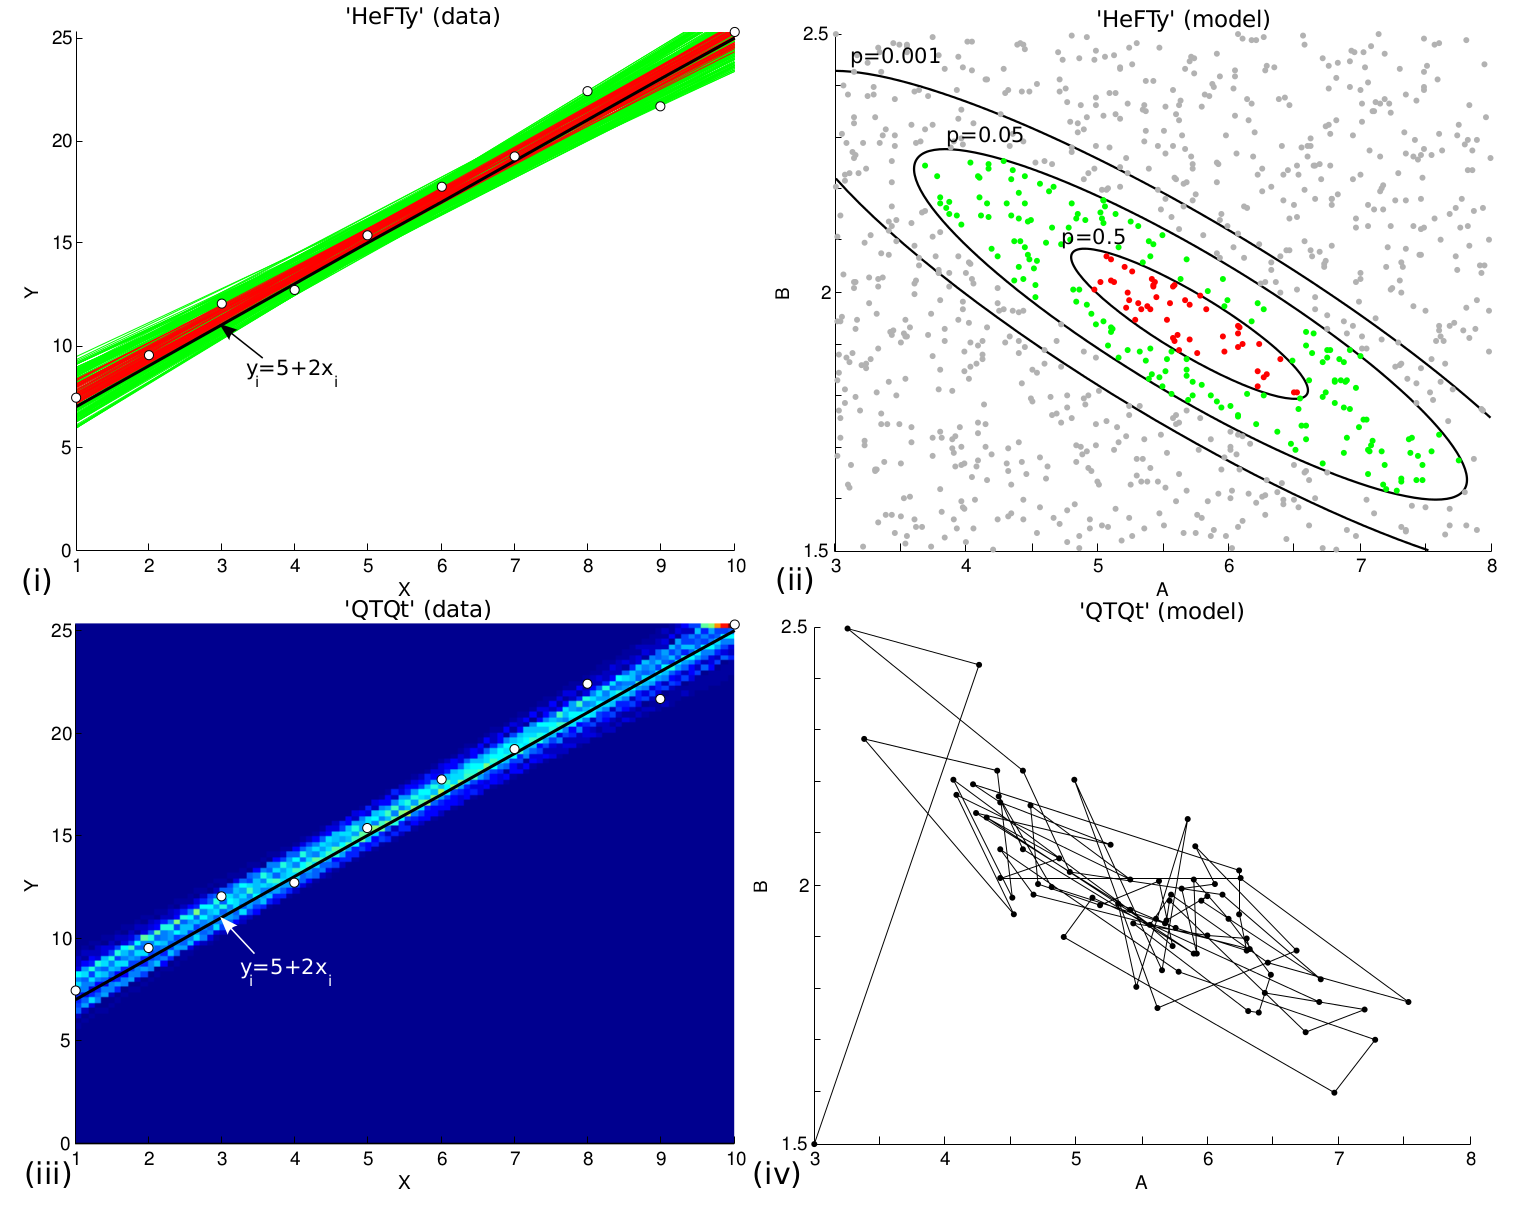
\includegraphics[width=\textwidth]{fig2.png}
\caption{(i) -- white circles show 10 data points drawn from a linear
  model (black line) with Normal residuals ($\sigma$=1).  Red and
  green lines show the linear trends that best fit the data according
  to the Chi-square test; (ii) -- the `Frequentist' Monte Carlo
  algorithm (`{\tt HeFTy}') makes 1000 independent random guesses for
  the intercept (A) and slope (B) drawn from a joint uniform
  distribution. A Chi-square goodness-of-fit test is done for each of
  these guesses. p-values $>$0.05 and and $>$0.5 are marked as green
  (`acceptable') and red (`good'), respectively. (iii) -- white
  circles and black line are the same as in (i). The colour of the
  pixels (ranging from blue to red) is proportional to the number of
  `acceptable' linear fits passing through them using the `Bayesian'
  algorithm (`{\tt QTQt}').  (iv) -- `{\tt QTQt}'makes a random walk
  (`Markov Chain') through parameter space, sampling the `posterior
  distribution' and yielding an `assemblage' of best fitting slopes
  and intercepts (black dots and lines).}
\label{fig:linear1}
\end{figure}

{\tt QTQt} also explores the `model space' by random sampling, but it
goes about this in a very different way than {\tt HeFTy}. Instead of
`carpet bombing' the parameter space with uniformly distributed
independent values, {\tt QTQt} performs a random walk of {\it serially
  dependent} random values. Starting from a random guess anywhere in
the parameter space, this `Markov Chain' of random models
systematically samples the model space so that models with high
$P(x,y|A_j,B_j)$ are more likely to be accepted than those with low
values. Thus, {\tt QTQt} bases the decision whether or not to accept
or reject the $j^{th}$ model not on the absolute value of
$P(x,y|A_j,B_j)$, but on the ratio of $P(x,y|A_j,B_j)$ /
$P(x,y|A_{j-1},B_{j-1})$.  See Appendix B for further details about
Markov Chain Monte Carlo (MCMC) modelling.  The important thing to
note at this point is that in well behaved systems like our linear
dataset, {\tt QTQt}'s MCMC approach yields identical results to {\tt
  HeFTy}'s Frequentist algorithm (Figure \ref{fig:linear1}(ii)-(iv)).


\subsection{Linear regression of weakly non-linear data}
\label{sec:nonlinear}

The physical models which geologists use to describe the diffusion of
helium or the annealing of fission tracks are but approximations of
reality.  To simulate this fact in our linear regression example, we
will now try to fit a linear model to a weakly non-linear dataset
generated using Equation \ref{eq:data} with a=5, b=2, c=0.02 and
$\sigma$=1. First, we consider a small sample of n=10 samples from
this distribution (Figure \ref{fig:linear2}(i)).  The quadratic term
(i.e., c) is so small that the naked eye cannot spot the non-linearity
of these data, and neither can `{\tt HeFTy}'. Using the same number of
N=1000 random guesses as before, `{\tt HeFTy}' finds 41 acceptable and
186 good fits using the $\chi^2$-test (Figure
\ref{fig:linear2}(ii)). In other words, with a sample size of n=10,
the non-linearity of the input data is `statistically insignificant'
relative to the data scatter $\sigma$.\\

\begin{figure}[!ht]
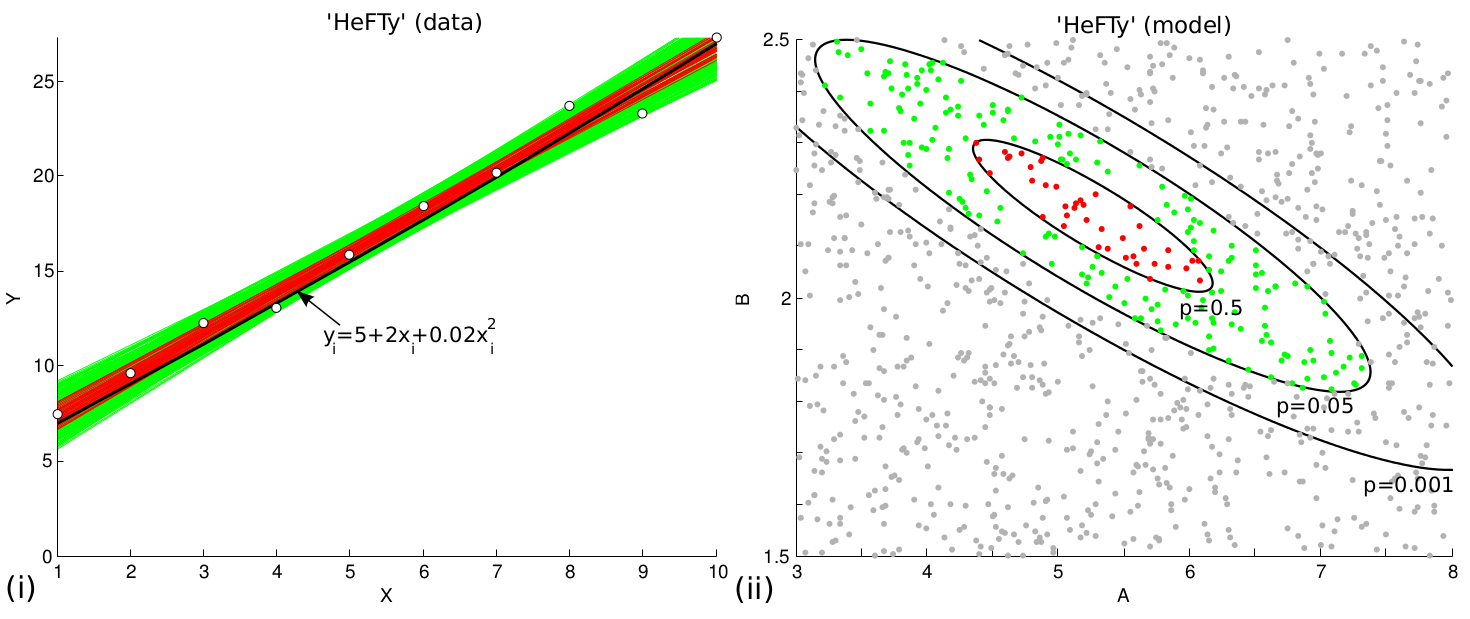
\includegraphics[width=\textwidth]{fig3.png}
\caption{(i) -- as Figure \ref{fig:linear1}(i) but using slightly
  non-linear input. (ii) -- as Figure \ref{fig:linear1}(ii): with a
  sample size of just 10 and relatively noisy data ($\sigma$=1) `{\tt
    HeFTy}' has no trouble finding best fitting linear models, and
  neither does `{\tt QTQt}' (not shown). }
\label{fig:linear2}
\end{figure}

The situation is very different when we increase the sample size to
n=100 (Figure \ref{fig:linear3}(i)-(ii)). In this case, `{\tt HeFTy}'
fails to find even a single linear model yielding a p-value greater
than 0.05. The reason for this is that the `power' of statistical
tests such as Chi-square increases with sample size (see Appendix C
for further details).  Even the smallest deviation from linearity
becomes `statistically significant' if a sufficiently large dataset is
available. This is important for thermochronology, as will be
illustrated in Section \ref{sec:breakingbad}. Similarly, the
statistical significance also increases with analytical
precision. Reducing $\sigma$ from 1 to 0.2 has the same effect as
increasing the sample size, as `{\tt HeFTy}' again fails to find any
`good' solutions (Figure \ref{fig:linear4}(i)-(ii)). `{\tt QTQt}', on
the other hand, handles the large (Figure \ref{fig:linear3}(iii)-(iv))
and precise (Figure \ref{fig:linear4}(iii)-(iv)) datasets much
better. In fact, increasing the quantity (sample size) or quality
(precision) of the data only has beneficial effects as it tightens the
solution space (Figure \ref{fig:linear3}(iv) vs.
\ref{fig:linear4}(iv)).

\begin{figure}[!ht]
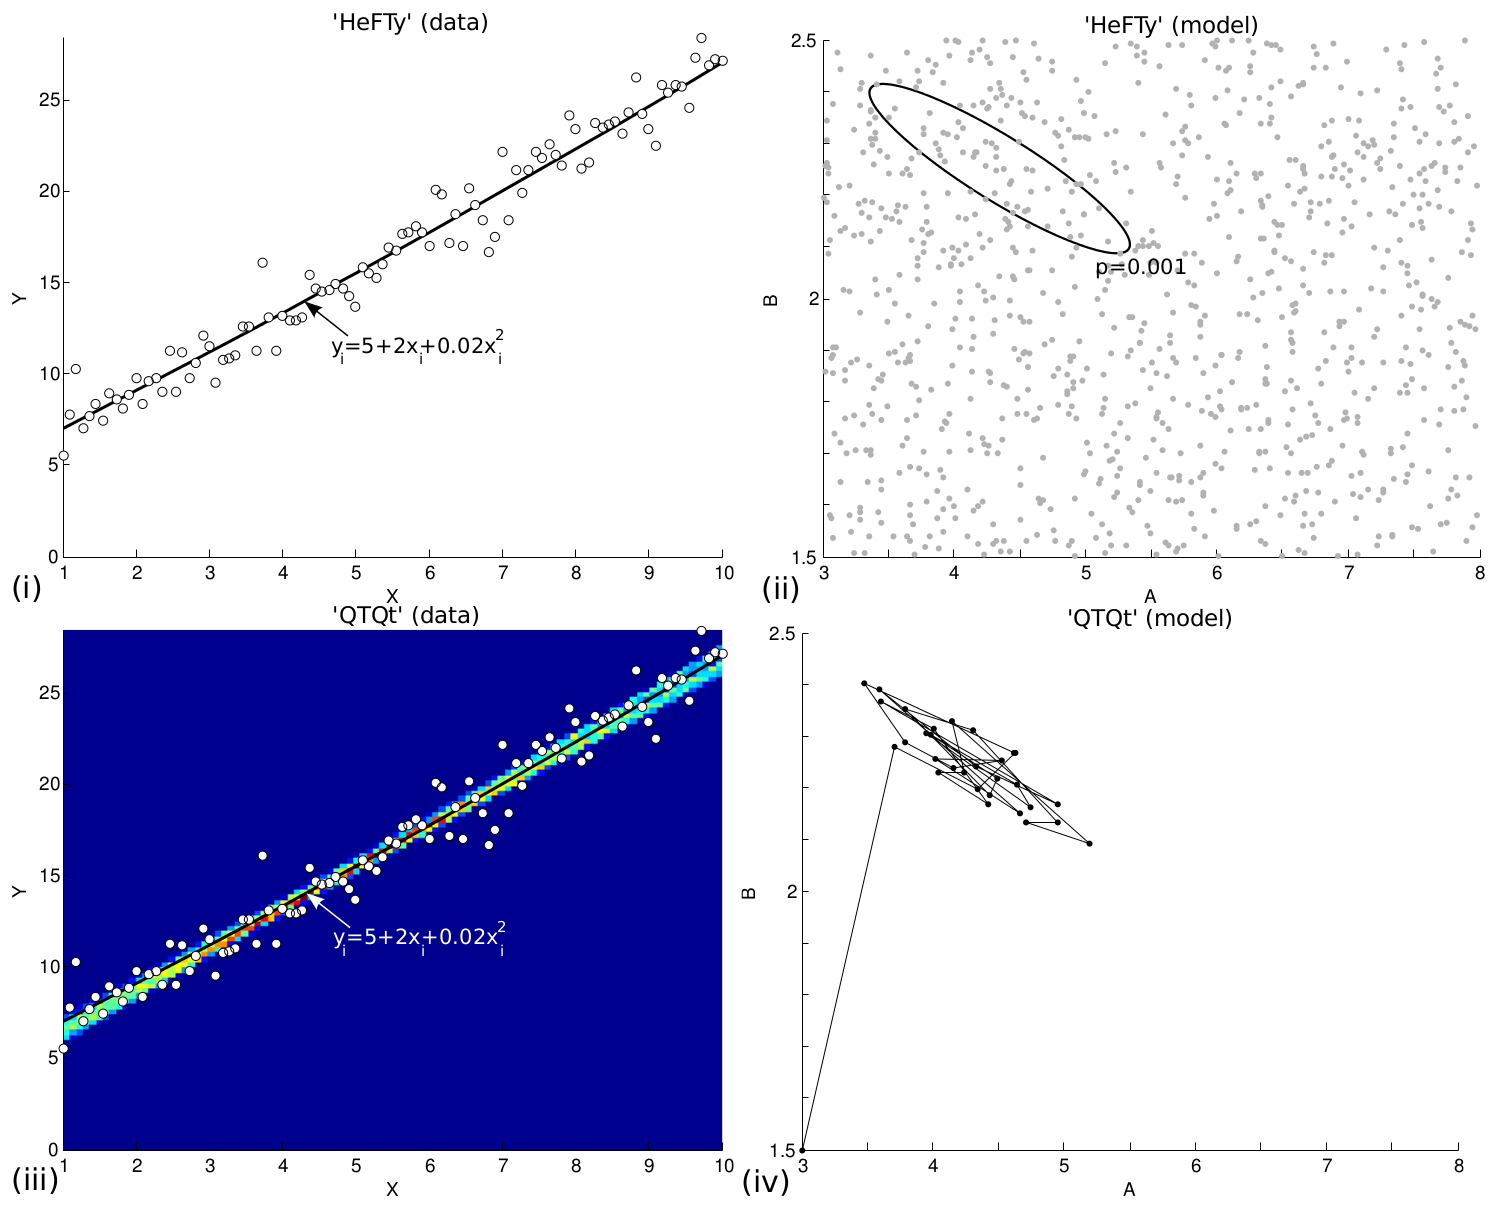
\includegraphics[width=\textwidth]{fig4.png}
\caption{(i)-(ii) as Figure \ref{fig:linear2}(i)-(ii) but with a
  sample size of 100: `{\tt HeFTy}' does not manage to find even a
  single `acceptable' linear fit to the data.  (iii)-(iv) -- the same
  data analysed by `{\tt QTQt}', which has no problems in finding a
  tight fit.}
\label{fig:linear3}
\end{figure}

\subsection{Linear regression of strongly non-linear data}
\label{sec:polynomial}

\begin{figure}[!ht]
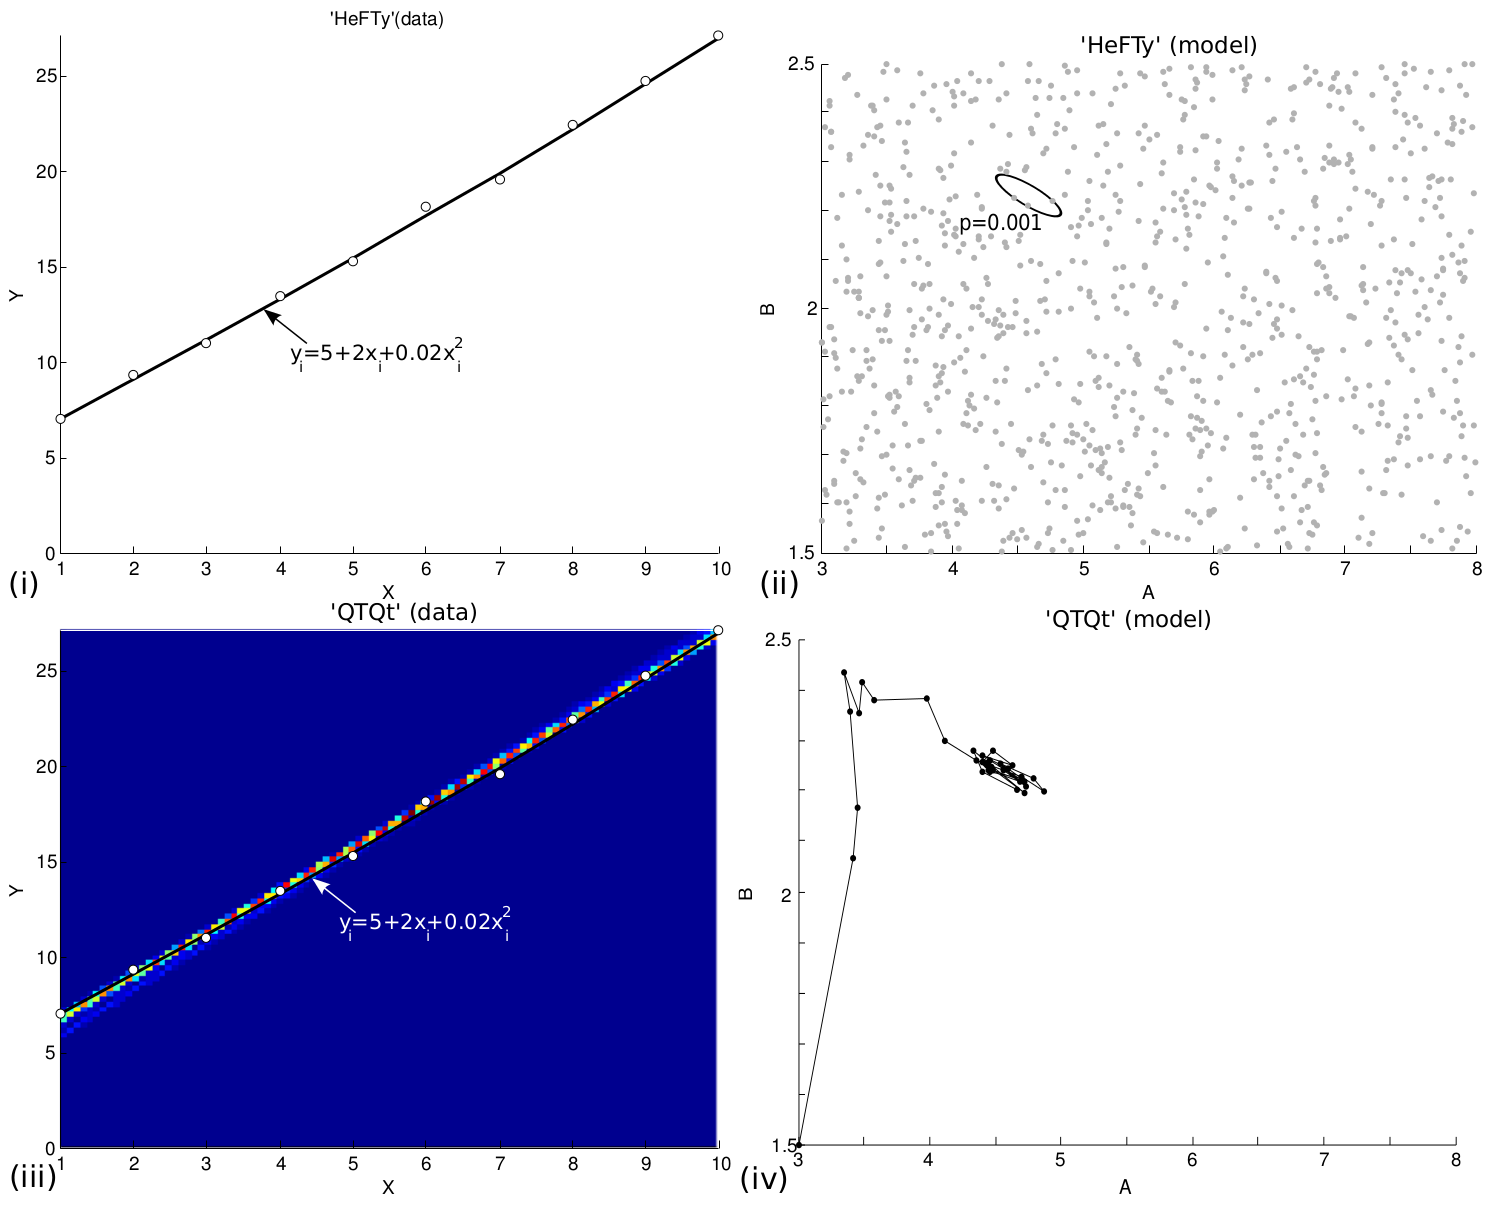
\includegraphics[width=\textwidth]{fig5.png}
\caption{(i)-(ii) -- as Figures \ref{fig:linear2}(i)-(ii) and
  \ref{fig:linear3}(i)-(ii) but with higher precision data
  ($\sigma$=0.2 instead of 1). Again, `{\tt HeFTy}' fails to find any
  `acceptable' solutions. (iii)-(iv) -- the same data analysed by
  `{\tt QTQt}', which works fine.}
\label{fig:linear4}
\end{figure}

For the third and final case study of our linear regression exercise,
consider a pathological dataset produced by setting a=26, b=-10, c=1
and $\sigma$=1. The resulting data points fall on a parabolic line,
which is far removed from the 2-parameter linear model of Equation
\ref{eq:model}. Needless to say, the `{\tt HeFTy}' algorithm does not
find any `acceptable' models. Nevertheless, the {\tt QTQt}-like MCMC
algorithm has no trouble fitting a straight line through these
data. Although the resulting likelihoods are orders of magnitude below
those of Figure \ref{fig:linear1}, their actual values are not used to
assess the goodness-of-fit, because the algorithm only evaluates the
relative ratios of the likelihood for adjacent models in the Markov
Chain (Appendix B).  It is up to the subjective judgement of the user
to decide whether to accept or reject the proposed inverse
models. This is very easy to do in the simple regression example of
this section, but may be significantly more complcated for
high-dimensional problems such as the thermal history modelling
discussed in the next section.  In conclusion, the simple linear
regression toy example has taught us that (a) the ability of a
Frequentist algorithm such as {\tt HeFTy} to find a suitable inverse
model critically depends on the quality {\it and} quantity of the
input data; while (b) the opposite is true for a Bayesian algorithm
like {\tt QTQt}, which always finds a suite of suitable models,
regardless how large or bad a dataset is fed into it.  The next
section of this paper will show that the same principles apply in
exactly the same way to thermochronology.

\begin{figure}[!ht]
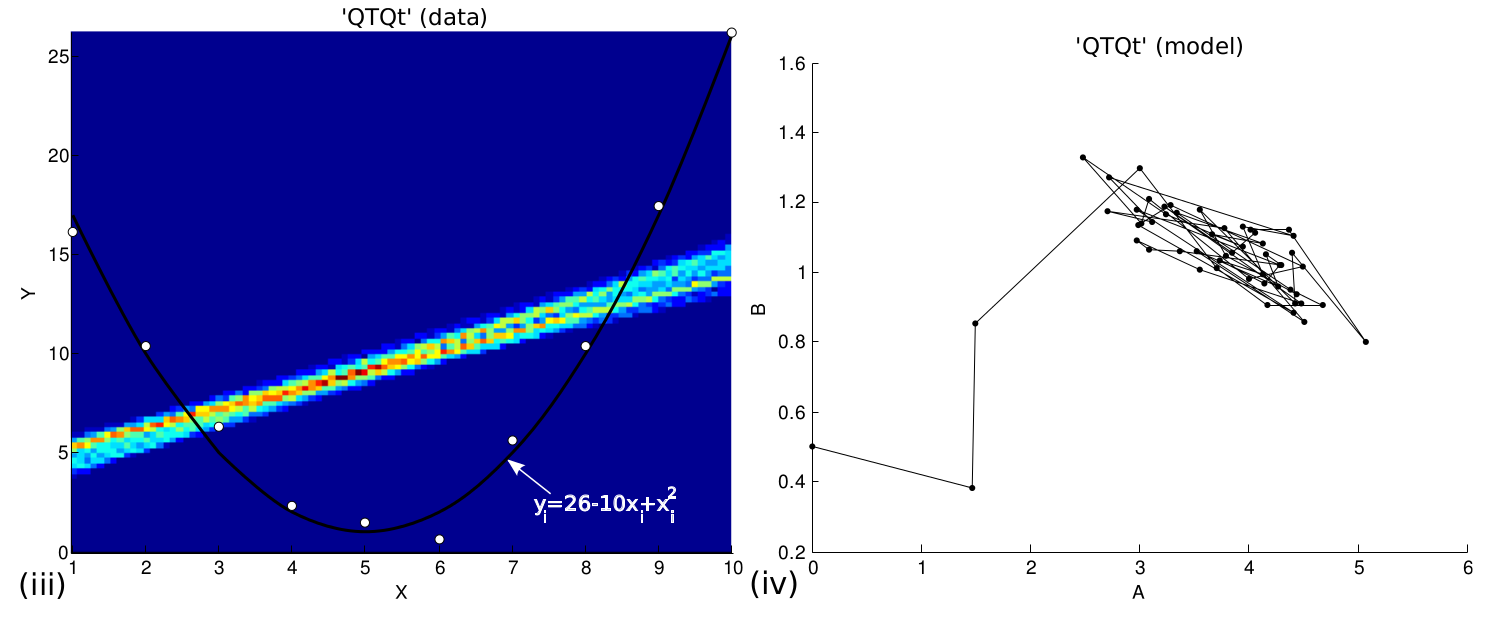
\includegraphics[width=\textwidth]{fig6.png}
\caption{(i) -- white circles show 10 data points drawn from a
  strongly non-linear model (black line). (ii) -- although it clearly
  does not make any sense to fit a straight line through these data,
  `{\tt QTQt}' nevertheless manages to do exactly that. `{\tt HeFTy}'
  (not shown), of course, does not.}
\label{fig:linear5}
\end{figure}

\section{Part II: thermal history modelling}
\label{sec:tTmodelling}

The previous section revealed significant differences between `{\tt
  HeFTy}-like' and `{\tt QTQt}-like' inverse modelling approaches to a
simple two-dimensional problem of linear regression.  Both algorithms
were shown to yield identical results in the presence of small and
well-behaved datasets. However, their response differed in response to
large or poorly behaved datasets. We will now show that exactly the
same phenomenon manifests itself in the multi-dimensional context of
thermal history modelling. First, we will use a geologically
straightforward thermochronological dataset to `break' {\tt HeFTy}
(Section \ref{sec:breakingbad}). Then, we will use a physically
impossible dataset to demonstrate that it is impossible to break {\tt
  QTQt} even when we want to (Section \ref{sec:garbage}).

\subsection{Large datasets `break' {\tt HeFTy}}
\label{sec:breakingbad}

We will investigate {\tt HeFTy} with a large but otherwise
unremarkable sample and using generic software settings like those
used by the majority of published {\tt HeFTy} applications.  The
sample (`KL29') was collected from a Mesozoic granite located in the
central Tibetan Plateau (GPS: 33.87N, 95.33E). It is characterised by
a 102 $\pm$ 7 Ma AFT age and a mean (unprojected) track length of
$\sim$12.1 $\mu$m, which was calculated from a dataset of 821
horizontally confined fission tracks. It is the large size of our
dataset that allows us to push {\tt HeFTy} to its limits. In addition
to the AFT data, we also measured five apatite U-Th-He (AHe) ages,
ranging from 47-66 Ma. AFT and AHe analyses were done at the
University of Melbourne and University College London using procedures
outlined by \cite{tian2014} and \cite{carter2014}, respectively.
For the thermal history modelling, we used the multi-kinetic annealing
model of \cite{ketcham2007}, employing Dpar as a kinetic
parameter. Helium diffusion in apatite was modelled with the Radiation
Damage Accumulation and Annealing Model (RDAAM) of
\cite{flowers2009}. Goodness-of-fit requirements for `good' and
`acceptable' thermal paths were defined as 0.5 and 0.05 (see Section
\ref{sec:linear}) and the present-day mean surface temperature was set
to 15 $\pm$ 15$^{\circ}$C. To speed up the inverse modelling, it was
necessary to specify a number of `bounding boxes' in time-temperature
(t-T) space.  The first of these t-T constraints was set at
140$^{\circ}$C/200Ma -- 20$^{\circ}$C/180Ma, i.e. slightly before the
oldest AFT age.  Five more equally broad boxes were used to guide the
thermal history modelling (Figure \ref{fig:Anti-HeFTy}). The issue of
`bounding boxes' will be discussed in more detail in Section
\ref{sec:boxes}.\\

In a first experiment, we modelled a small subset of our data
comprising just the first 100 track length measurements. After one
million iterations, {\tt HeFTy} returned 39 `good' and 1,373
`acceptable' thermal histories, featuring a poorly resolved phase
prior to 120 Ma, followed by rapid cooling to $\sim$60$^\circ$C, a
protracted isothermal residence in the upper part of the AFT partial
annealing zone from 120-40 Ma, and ending with a phase of more rapid
cooling from 60 to 15$^{\circ}$C since 40 Ma. This is in every way an
unremarkable thermal history, which correctly reproduces the
negatively skewed (c-axis projected) track length distribution, and
predicts AFT and AHe ages of 102 and 59 Ma, respectively, well within
the range of the input data (Figure \ref{fig:Anti-HeFTy}(i)).  Next,
we move on to a larger dataset, which was generated using the same AFT
and AHe ages as before, but measuring an extra 269 confined fission
tracks in the same slide as the previously measured 100
tracks. Despite the addition of so many extra measurements, the
resulting length distribution looks very similar to the smaller
dataset. Nevertheless, {\tt HeFTy} struggles to find suitable thermal
histories. In fact, the program fails to find a single `good' t-T path
even after a million iterations, and only comes up with a measly 109
`acceptable' solutions. A closer look at the model predictions reveals
that {\tt HeFTy} does a decent job at modelling the track length
distribution, but that this comes at the expense of the AFT and AHe
age predictions, which are further removed from the measured values
than in the small dataset (Figure \ref{fig:Anti-HeFTy}(ii)). In a
final experiment, we prepared a second fission track slide for sample
KL29, yielding a further 452 fission track length measurements. This
brings the total tally of the length distribution to an unprecedented
821 measurements, allowing us to push {\tt HeFTy} to its breaking
point. After one million iterations, {\tt HeFTy} does not manage to
find even a single `acceptable' t-T path (Figure
\ref{fig:Anti-HeFTy}(iii)).  \\

It is troubling that {\tt HeFTy} performs worse for large datasets
than it does for small ones. It seems unfair that the user should be
penalised for the addition of extra data. The reasons for this
behaviour will be discussed in Section \ref{sec:discussion}.  But
first, we shall have a closer look at {\tt QTQt}, which has no problem
fitting the large dataset (Figure \ref{fig:Anti-QTQt}(i)) but poses
some completely different challenges.

\begin{figure}[!ht]
\centering
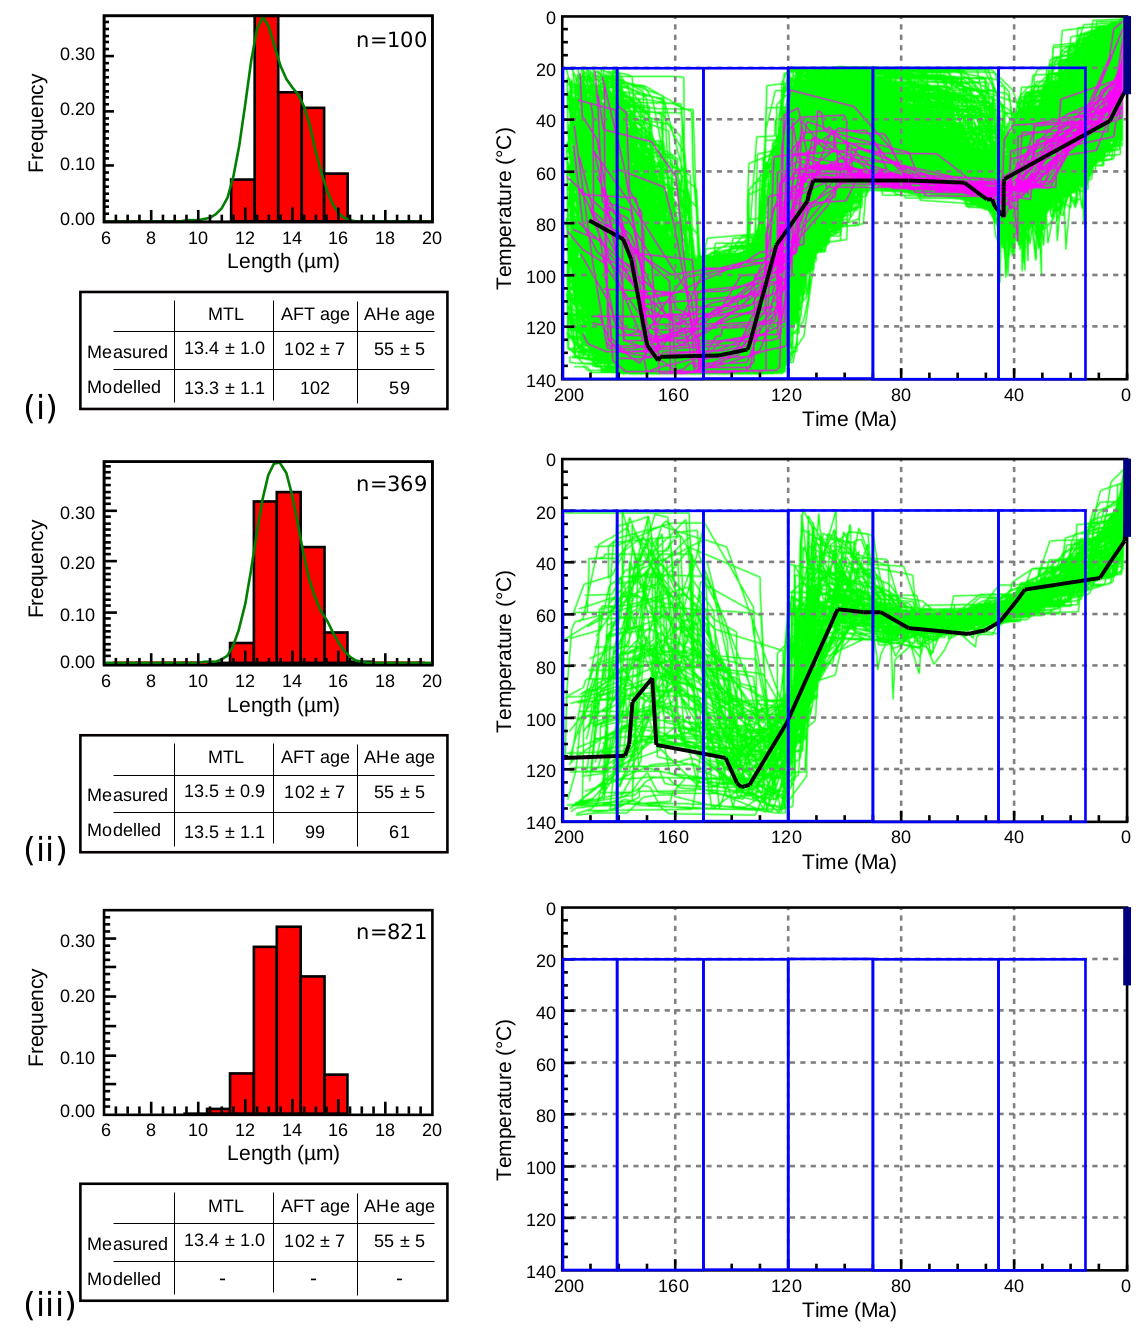
\includegraphics[width=\textwidth]{fig7.png}
\caption{Data (left column) and inverse model solutions (right column)
  produced by {\tt HeFTy} [v1.8.2, \cite{ketcham2005}] for sample
  KL29. (c-axis projected) track length distributions are shown as
  histograms. Bounding boxes (blue) were used to reduce the model
  space and speed up the inverse modelling (Section
  \ref{sec:boxes}). (i) -- red and green time temperature (t-T) paths
  mark `good' and `acceptable' fits to the data, corresponding to
  p-values of 0.5 and 0.05, respectively. (ii) -- as the number of
  track length measurements (n) increases, p-values decrease (for
  reasons given in Appendix C) and {\tt HeFTy} struggles to find
  acceptable solutions. (iii) -- eventually, when n=821, the program
  `breaks'.}
\label{fig:Anti-HeFTy}
\end{figure}

\subsection{`garbage in, garbage out' with {\tt QTQt}}
\label{sec:garbage}

Contrary to {\tt HeFTy}, {\tt QTQt} does not mind large datasets. In
fact, its inverse modelling results improve with the addition of more
data. This is because large datasets allow the `reversible jump MCMC'
algorithm (Appendix B) to add more anchor points to the candidate
models, thereby improving the resolution of the t-T history. Thus,
{\tt QTQt} does not punish but reward the user for adding data. For
the full 821-length dataset of KL29, this results in a thermal history
similar to the {\tt HeFTy} model of Figure \ref{fig:Anti-HeFTy}(i). We
therefore conclude that {\tt QTQt} is much more robust than {\tt
  HeFTy} in handling large and possible complex datasets. However,
this greater robustness also carries a danger with it, as will be
shown next. We now apply {\tt QTQt} to a semi-synthetic dataset
generated by arbitrarily changing the AHe age of sample KL29 from 55
$\pm$ 5 Ma to 102 $\pm$ 7 Ma, i.e. identical to its AFT age.  As
discussed in Section \ref{sec:breakingbad}, the sample has a short
($\sim$12.1 $\mu$m) mean (unprojected) fission track length,
indicating slow cooling through the AFT partial annealing zone.  The
identical AFT and AHe ages, however, imply infinitely rapid cooling.
The combination of the AFT and AHe data is therefore physically
impossible and, not surprisingly, {\tt HeFTy} fails to find a single
`acceptable' fit even for a moderate sized dataset of 100 track
lengths.  {\tt QTQt}, however, has no problem finding a `most likely'
solution (Figure \ref{fig:Anti-QTQt}(ii)).\\

The resulting assemblage of models is characterised by a long period
of isothermal holding at the base of the AFT partial annealing zone
($\sim$120 $^{\circ}$C), followed by rapid cooling at 100Ma, gentle
heating to the AHe partial retention zone ($\sim$60 $^{\circ}$C) until
20 Ma and rapid cooling to the surface thereafter (Figure
\ref{fig:Anti-QTQt}(ii)). This assemblage of thermal history models is
largely unremarkable and does not, in itself, indicate any problems
with the input data. These problems only become clear when we compare
the measured with the modelled data. While the fit to the track length
measurements is good, the AFT and AHe ages are off by 20\%. It is then
up to the user to decide whether or not this is `significant' enough
to reject the model results.  This is not necessarily as
straightforward as it may seem.  For instance, the original {\tt QTQt}
paper by [Figure 7, \cite{gallagher2012}] presents a dataset in which
the measured and modelled values for the kinetic parameter DPar differ
by 25\%. In this case, the author has made a subjective decision to
attach less credibility to the DPar measurement. This may very well be
(and probably is) justified, but nevertheless requires expert
knowledge of thermochronology while remaining, once again,
subjective. This subjectivity is the price of Bayesian MCMC modelling.

\begin{figure}[!ht]
\centering
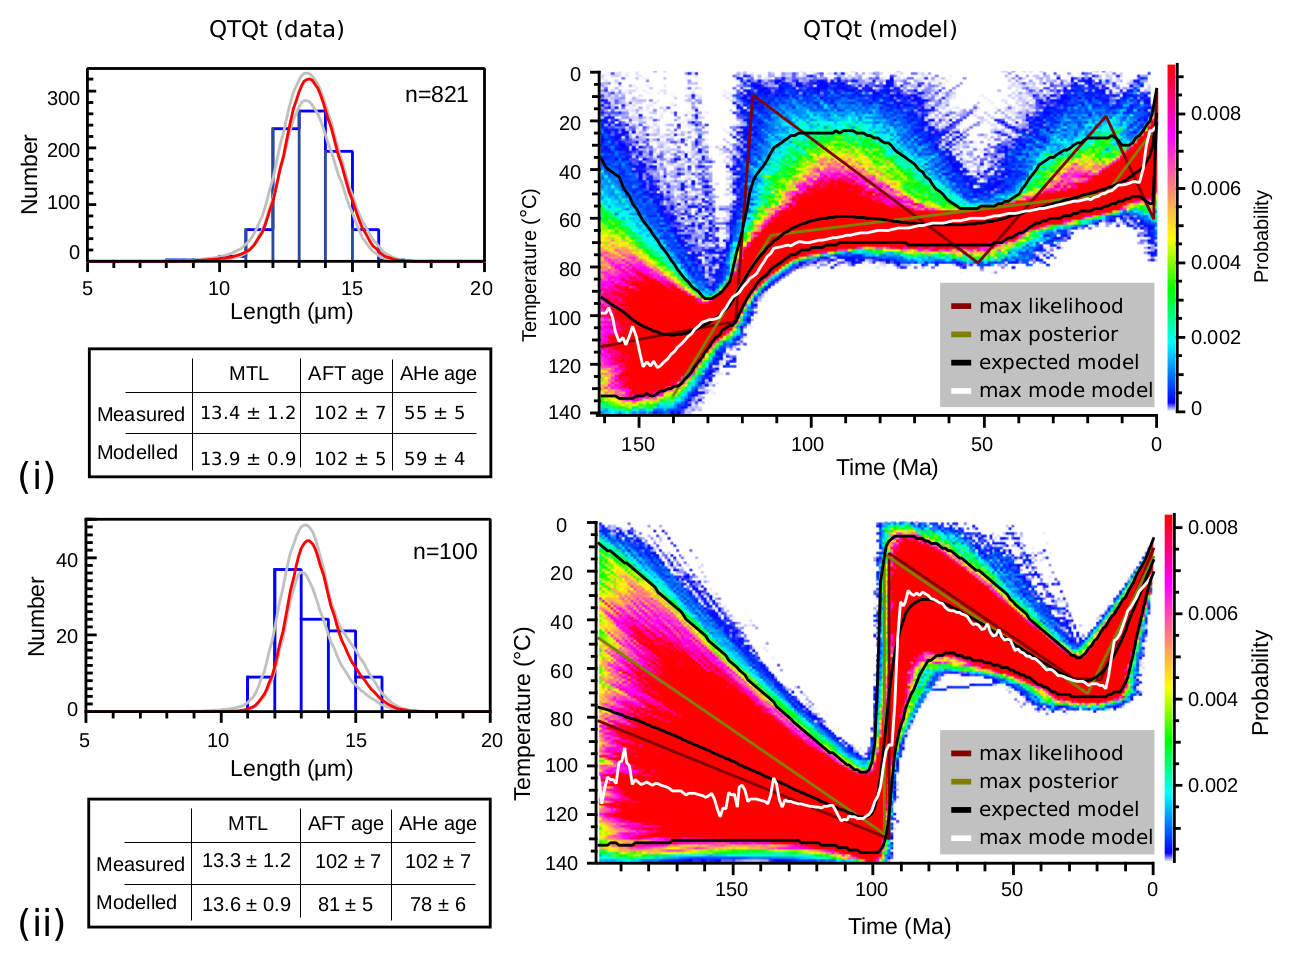
\includegraphics[width=\textwidth]{fig8.png}
\caption{Data (left) and models (right) produced by {\tt QTQt}
  [v4.5, \cite{gallagher2012}], after a `burn-in' period of 500,000
  iterations, followed by another 500,000 `post-burn-in' iterations.
  No time or temperature constraints were given apart from a broad
  search limit of 102 $\pm$ 102 Ma and 70 $\pm$ 70 $^\circ$C.  (i) --
  {\tt QTQt} has no trouble fitting the large dataset that broke {\tt
    HeFTy} in Figure \ref{fig:Anti-HeFTy}.  (ii) -- neither does {\tt
    QTQt} complain when a physically impossible dataset with short
  fission tracks and identical AFT and AHe ages is fed into it. Note
  that the `measured' mean track lengths reported in this table are
  slightly different from those of Figure \ref{fig:Anti-HeFTy},
  despite being based on exactly the same data.  This is because {\tt
    QTQt} calculates the c-axis projected values using an average Dpar
  for all lengths, whereas {\tt HeFTy} uses the relevant Dpar for each
  length.}
\label{fig:Anti-QTQt}
\end{figure}

\section{Discussion}
\label{sec:discussion}

The behaviour shown by {\tt HeFTy} and {\tt QTQt} in a
thermochronological context (Section \ref{sec:tTmodelling}) is
identical to the toy example of linear regression (Section
\ref{sec:regression}). {\tt HeFTy} is `too picky' when it comes to
large datasets and {\tt QTQt} is `not picky enough' when it comes to
bad datasets. These opposite types of behaviour are a direct
consequence of the statistical underpinnings of the two programs.  The
sample size dependence of {\tt HeFTy} is caused by the fact that it
judges the merits of the trial models by means of formalised
statistical hypothesis tests, notably the Kolmogorov-Smirnov (K-S) and
$\chi^2$-tests. These tests are designed to make a black or white
decision as to whether the hypothesis is right or wrong.  However, as
stated in Section \ref{sec:nonlinear}, the physical models produced by
Science (including Geology) are ``but approximations of reality'' and
are therefore always `somewhat wrong'.  This should be self-evident
from a brief look at the Settings menu of {\tt HeFTy}, which offers
the user the choice between, for example, the kinetic annealing model
of \cite{laslett1987} or \cite{ketcham2007}. Surely it is logically
impossible for both models to be correct. Yet for sufficiently small
samples, {\tt HeFTy} will find plenty of `good' t-T paths in both
cases. The truth of the matter is that both the \cite{laslett1987}
and the \cite{ketcham2007} models are incorrect, albeit to different
degrees. As sample size increases, the `power' of statistical tests
such as K-S and $\chi^2$ to detect the `wrongness' of the annealing
models increases as well (Appendix C).  Thus, as we keep adding
fission track length measurements to our dataset, {\tt HeFTy} will
find it more and more difficult to find `acceptable' t-T
paths. Suppose, for the sake of the argument, that the
\cite{laslett1987} annealing model is `more wrong' than the
\cite{ketcham2007} model. This will manifest itself in the fact that
beyond a critical sample size, {\tt HeFTy} will fail to find even a
single `acceptable' model using the \cite{laslett1987} model, while
the \cite{ketcham2007} model will still yield a small number of
`non-disprovable' t-T paths. However, if we further increase the
sample size beyond this point, then even the \cite{ketcham2007} model
will eventually fail to yield any `acceptable' solutions.\\

The problem is that Geology itself imposes unrealistic assumptions on
our thermal modelling efforts. Our understanding of diffusion and
annealing kinetics is based on short term experiments carried out in
completely different environments than the geological processes which
we aim to understand. For example, helium diffusion experiments are
done under ultra-high vacuum at temperatures of hundreds of degrees
over a duration of at most a few weeks. These are very different
conditions than those found in the natural environment, where
diffusion takes place under hydrostatic pressure at a few tens of
degrees over millions of years \cite{villa2006}. But even if we
disregard this problem, and imagine a utopian scenario in which our
annealing and diffusion models are an exact description of reality,
the p-value conundrum would persist, because there are dozens of other
experimental factors that can go wrong, resulting in dozens of reasons
for K-S and $\chi^2$ to reject the data. Examples are observer bias in
AFT analysis \cite{ketcham2009} or inaccurate $\alpha$-ejection
correction due to undetected U-Th-zonation in AHe dating
\cite{hourigan2005}.  Given a large enough data set, K-S and $\chi^2$
will be able to `see' these effects.\\

One apparent solution to this problem is to adjust the p-value cutoffs
for `good' and `acceptable' models from their default values of 0.5
and 0.05 to another value, in order to account for differences in
sample size. Thus, large datasets would require lower p-values than
small ones. The aim of such a procedure would be to objectively accept
or reject models based on a sample-independent `effect size' (see
Appendix C). Although this sounds easy enough in theory, the
implementation details are not straightforward.  The problem is that
{\tt HeFTy} is very flexible in accepting many different types of data
and it is unclear how these can be normalised in a common reference
frame.  For example, one data set might include only AFT data, a
second AFT as well as AHe data, while a third might throw some
vitrinite reflectance data into the mix as well. Each of these
different types of data is evaluated by a different statistical test,
and it is unclear how to consistently account for sample size in this
situation. On a related note, it is important to discuss the current
way in which {\tt HeFTy} combines the p-values for each of the
previously mentioned hypothesis tests. Sample KL29 of Section
\ref{sec:tTmodelling}, for example, yields three different p-values:
one for the fission track lengths, one for the AFT ages and one for
the AHe ages. {\tt HeFTy} bases the decision whether to reject or
accept a t-T path based on the lowest of these three values
\cite{ketcham2005}. This causes a second level of problems, as the
chance of erroneously rejecting a correct null hypothesis (a so-called
`Type-I error') increases with the number of simultaneous hypothesis
tests. In this case we recommend that the user adjust the p-value
cutoff by dividing it by the number of datasets (i.e., use a cutoff of
0.5/3 = 0.17 for `good' and 0.05/3 = 0.017 for `acceptable'
models). This is called the `Bonferroni correction' [e.g., p.424
  of \cite{rice1995}].\\

In summary, the very idea to use statistical hypothesis tests to
evaluate the model space is problematic. Unfortunately, we cannot use
p-values to make a reliable decision to find out whether a model is
`good' or `acceptable', independent of sample size. {\tt QTQt} avoids
this problem by \emph{ranking} the models from `bad' to `worse', and
then selecting the `most likely' ones according to the posterior
probability (Appendix A). Because the MCMC algorithm employed by {\tt
  QTQt} only determines the posterior probability up to a
multiplicative constant, it does not care `how bad' the fit to the
data is. The advantage of this approach is that it always produces
approximately the same number of solutions, regardless of sample
size. The disadvantage is that the ability to automatically detect and
reject faulty datasets is lost.  This may not be a problem, one might
think, if sufficient care is taken to ensure that the analytical data
are sound and correct. However, that does not exclude the possibility
that there are flaws in the forward modelling routines. For example,
recall the two fission track annealing models previously mentioned in
Section \ref{sec:discussion}. Although the \cite{ketcham2007} model
may be a better representation of reality than the \cite{laslett1987}
model and, therefore, yield more `good' fits in {\tt HeFTy}, the
difference would be invisible to {\tt QTQt} users. The program will
always yield an assemblage of t-T models, regardless of the annealing
model used.  As a second example, consider the poor age
reproducibility that characterises many U-Th-He datasets and which has
long puzzled geochronologists \cite{fitzgerald2006}. A number of
explanations have been proposed to explain this dispersion over the
years, ranging from invisible and insoluble actinide-rich mineral
inclusions \cite{vermeesch2007b}, $\alpha$-implantation by `bad
neighbours' \cite{spiegel2009}, fragmentation during mineral
separation \cite{brown2013} and radiation damage due to
$\alpha$-recoil \cite{flowers2009}. The latter two hypotheses are
linked to precise forward models which can easily be incorporated into
inverse modelling software such as {\tt HeFTy} and {\tt QTQt}. Some
have argued that dispersed data are to be preferred over non-dispersed
measurements because they offer more leverage for t-T modelling
\cite{beucher2013}.  However, all this assumes that the physical
models are correct, which, given the fact that there are so many
competing `schools of thought', is unlikely to be true in all
situations. Nevertheless, {\tt QTQt} will take whatever assumption
specified by the user and run with it. It is important to note that
{\tt HeFTy} is not immune to these problems either. Because
sophisticated physical models such as RDAAM comprise many additional
parameters and, hence, `degrees of freedom', the statistical tests
used by {\tt HeFTy} are easily underpowered (Appendix C), yielding
many `good' solutions and producing a false sense of confidence in the
inverse modelling results.\\

In conclusion, the evaluation of whether an inverse model is
physically sound is more subjective in {\tt QTQt} than it is in {\tt
  HeFTy}. There is no easy way to detect analytical errors or invalid
model assumptions other than by subjectively comparing the predicted
data with the input measurements.  Note that it is possible to `fix'
this limitation of {\tt QTQt} by explicitly evaluating the
multiplicative constant given by the denominator in Bayes' Theorem
(Appendix A). We could then set a cutoff value for the posterior
probability to define `good' and `acceptable' models, just like in
{\tt HeFTy}. However, this would cause exactly the same problems of
sample size dependency as we saw earlier.  Conversely, {\tt HeFTy}
could be modified in the spirit of {\tt QTQt}, by using the p-values
to {\it rank} models from `bad' to `worst', and then simply plotting
the `most likely' ones.  Unfortunately, the problem with this approach
is the sensitivity of {\tt HeFTy} to the dimensionality of the model
space. In order to be able to objectively compare two samples using
the proposed ranking algorithm, the parameter space should be devoid
of `bounding boxes', and be fixed to a constant search range in time
and temperature. This would make {\tt HeFTy} unreasonably slow, for
reasons explained in Section \ref{sec:boxes}.


\section{On the selection of time-temperature constraints}
\label{sec:boxes}

As we saw in Section \ref{sec:breakingbad}, {\tt HeFTy} allows, and
generally even requires, the user to constrain the search space by
means of `bounding boxes'.  Often these boxes are chosen to correspond
to geological constraints, such as known phases of surface exposure
inferred from independently dated unconformities. But even when no
formal geological constraints are available, the program often still
requires bounding boxes to speed up the modelling.  This is a
manifestation of the so-called `curse of dimensionality', which is a
problem caused by the exponential increase in `volume' associated with
adding extra dimensions to a mathematical space. Consider, for
example, a unit interval. The average nearest neighbour distance
between 10 random samples from this interval will be 0.1. To achieve
the same sampling density for a unit square requires not 10 but 100
samples, and for a unit cube 1000 samples.  The parameter space
explored by {\tt HeFTy} comprises not two or three but commonly dozens
of parameters (i.e., anchor points in time-temperature space),
requiring tens of thousands of uniformly distributed random sets to be
explored in order to find the tiny subset of statistically plausible
models.  Furthermore, the `sampling density' of {\tt HeFTy}'s randomly
selected t-T paths also depends on the allowed range of time and
temperature. For example, keeping the temperature range equal, it
takes twice as long to sample a t-T space spanning 200 Myr than one
spanning 100 Myr. Thus, old samples tend to take much longer to model
than young ones. The only way for {\tt HeFTy} to get around this
problem is by shrinking the search space. One way to do this is to
only permit monotonically rising t-T paths. Another is to use
`bounding boxes', like in Section \ref{sec:breakingbad} and Figure
\ref{fig:Anti-HeFTy}.  It is important not to make these boxes too
small, especially when they are derived from geological
constraints. Otherwise the set of `acceptable' inverse models may
simply connect one box to the next, mimicking the geological
constraints without adding any new geological insight.\\

The curse of dimensionality affects {\tt QTQt} in a different way than
{\tt HeFTy}. As explained in Section \ref{sec:regression}, {\tt QTQt}
does not explore the multi-dimensional parameter space by means of
independent random uniform guesses, but by performing a random walk
which explores just a small subset of that space. Thus, an increase in
dimensionality does not significantly slow down {\tt QTQt}. However,
this does not mean that {\tt QTQt} is insensitive to the
dimensionality of the search space. The `reversible jump MCMC'
algorithm allows the number of parameters to vary from one trial model
to the next (Appendix B). To prevent spurious overfitting of the data,
this number of parameters is usually quite low. Whereas {\tt HeFTy}
commonly uses ten or more anchor points (i.e. $>$20 parameters) to
define a t-T path, {\tt QTQt} uses far fewer than that. For example,
the maximum likelihood models in Figure \ref{fig:Anti-QTQt} use just
three and six t-T anchor points for the datasets comprising 100 and
821 track lengths, respectively. The crudeness of these models is
masked by averaging, either through the graphical trick of
colour-coding the number of intersecting t-T paths, or by integrating
the model assemblages into `maximum mode' and `expected' models
\cite{sambridge2006, gallagher2012}. It is not entirely clear how
these averaged models relate to physical reality, but a thorough
discussion of this subject falls outside the scope of this
paper. Instead, we would like to redirect our attention to the subject
of `bounding boxes'.\\

Although {\tt QTQt} does allow the incorporation of geological
constraints, we would urge the user to refrain from using this
facility for the following reason.  As we saw in Sections
\ref{sec:nonlinear} and \ref{sec:garbage}, {\tt QTQt} always finds a
`most likely' thermal history, even when the data are physically
impossible. Thus, in contrast with {\tt HeFTy}, {\tt QTQt} cannot be
used to \emph{disprove} the geological constraints. We would argue
that this, in itself, is reason enough not to use `bounding boxes' in
{\tt QTQt}. Incidentally, we would also like to make the point that,
to our knowledge, no thermal history model has ever been shown to
independently reproduce known geological constraints such as a well
dated unconformity followed by burial.  Such empirical validation is
badly needed to justify the degree of faith many users seem to have in
interpreting subtle details of thermal history models.  This point
becomes ever more important as thermochronology is increasingly being
used outside the academic community, and is affecting business
decisions in, for example, the hydrocarbon industry.

\section{Conclusions}

There are three differences between the methodology used by {\tt
  HeFTy} and {\tt QTQt}:

\begin{enumerate} 
\item {\tt HeFTy} is a `Frequentist' algorithm which evaluates the
  likelihood P(x,y$|$A,B) of the data (\{x,y\}, e.g. two-dimensional
  plot coordinates in Section \ref{sec:regression} or AFT and AHe data
  in Section \ref{sec:tTmodelling}) given the model (\{A,B\}, e.g.,
  slopes and intercepts in Section \ref{sec:regression} or anchor
  points of t-T paths in Section \ref{sec:tTmodelling}).  {\tt QTQt},
  on the other hand, follows a `Bayesian' paradigm in which inferences
  are based on the posterior probability P(A,B$|$x,y) of the model
  given the data (Appendix A).
\item {\tt HeFTy} evaluates the model space (i.e., the set of all
  possible slopes in Section \ref{sec:regression}, or all possible t-T
  paths in Section \ref{sec:tTmodelling}) using mutually independent
  random uniform draws. In contrast, {\tt QTQt} explores the model
  space by collecting an assemblage of serially dependent random
  models over the course of a random walk (Appendix B).
\item {\tt HeFTy} accepts or rejects candidate models based on the
  actual value of the likelihood, via a derived quantity called the
  `p-value' (Appendix C). {\tt QTQt} simply ranks the models in
  decreasing order of posterior probability and plots the most likely
  ones.
\end{enumerate}

Of these three differences, the first one (`Frequentist'
vs. `Bayesian') is actually the least important. In fact, one
could easily envisage a Bayesian algorithm which behaves identical to
{\tt HeFTy}, by explicitly evaluating the posterior probability, as
discussed in Section \ref{sec:discussion}.  Conversely, in the
regression example of Section \ref{sec:regression}, the posterior
probability is proportional to the likelihood, so that one would be
justified in calling the resulting MCMC model `Frequentist'.  The
second and third difference between {\tt HeFTy} and {\tt QTQt} are
much more important.  Even though {\tt HeFTy} and {\tt QTQt} produce
similar looking assemblages of t-T paths, the statistical meaning of
these assemblages is fundamentally different. The output of {\tt
  HeFTy} comprises \emph{``all those t-T paths which cannot be
  rejected with the available evidence''}. In contrast, the
assemblages of t-T paths generated by {\tt QTQt} contain \emph{``the
  most likely t-T paths, assuming that the data are good and the model
  assumptions are appropriate''}. The difference between these two
definitions goes much deeper than mere semantics.  It reveals a
fundamental difference in the way the model results of both programs
ought to be interpreted. In the case of {\tt HeFTy}, a `successful'
inversion yielding many `good' and `acceptable' t-T paths may simply
indicate that there is insufficient evidence to extract meaningful
thermal history information from the data. As for {\tt QTQt}, its t-T
reconstructions are effectively meaningless unless they are plotted
alongside the input data and model predictions.  \\

{\tt HeFTy} is named after a well known brand of waste disposal bags,
as a welcome reminder of the `garbage in, garbage out' principle.
{\tt QTQt}, on the other hand derives its name from the ability of
thermal history modelling software to extract colourful and easily
interpretable time-temperature histories from complex analytical
datasets\footnote{Additionally, `Qt' also refers to the cross-platform
  application framework used for the development of the software.}.
In light of the observations made in this paper, it appears that the
two programs have been `exchanged at birth', and that their names
should have been swapped.  First, {\tt HeFTy} is an arguably easier to
use and visually more appealing (`cute') piece of software than {\tt
  QTQt}.  Second, and more importantly, {\tt QTQt} is more prone to
the `garbage in, garbage out' problem than {\tt HeFTy}. By using
p-values, {\tt HeFTy} contains a built-in quality control mechanism
which can protect the user from the worst kinds of `garbage' data. For
example, the physically impossible dataset of Section
\ref{sec:garbage} was `blocked' by this safety mechanism and yielded
no `acceptable' thermal history models in {\tt HeFTy}. However, in
normal to small datasets, the statistical tests used by {\tt HeFTy}
are often underpowered and the `garbage in, garbage out' principle
remains a serious concern. Nevertheless, {\tt HeFTy} is less
susceptible to overinterpretation than {\tt QTQt}, which lacks an
`objective' quality control mechanism. It is up to the expertise of
the analist to make a subjective comparison between the input data and
the model predictions made by {\tt QTQt}.\\

Unfortunately, and this is perhaps the most important conclusion of
our paper, {\tt HeFTy}'s efforts in dealing with the `garbage' data
come at a high cost.  In its attempt to make an `objective' evaluation
of candidate models, {\tt HeFTy} acquires an undesirable sensitivity
to sample size.  {\tt HeFTy}'s power to resolve even the tiniest
violations of the model assumptions increases with the amount and the
precision of the input data.  Thus, as was shown in a regression
context (Section \ref{sec:nonlinear} and Figure \ref{fig:linear2}) as
well as thermochronology (Section \ref{sec:tTmodelling} and Figure
\ref{fig:Anti-HeFTy}), {\tt HeFTy} will fail to come up with even a
single `acceptable' model if the analytical precision is very high or
the sample size is very large.  Put in another way, the ability of
{\tt HeFTy} extract thermal histories from AFT and AHe
\cite{tian2014}, apatite U-Pb \cite{cochrane2014} or $^4$He/$^3$He
data \cite{karlstrom2014} only exists by virtue of the relative
sparsity and low analytical precision of the input data. It is
counter-intuitive and unfair that the user should be penalised for
acquiring large and precise datasets. In this respect, the MCMC
approach taken by {\tt QTQt} is more sensible, as it does not punish
but reward large and precise datasets, in the form of more detailed
and tightly constrained thermal histories.  Although the inherent
subjectivity of {\tt QTQt}'s approach may be perceived as a negative
feature, it merely reflects the fact that thermal history models
should always be interpreted in a wider geological context.  What is
`significant' in one geological setting may not necessarily be so in
another, and no computer algorithm can reliably make that call on
behalf of the geologist. As George Box famously said, ``all models are
wrong, but some are useful''.

\section*{Appendix A: Frequentist vs. Bayesian inference}

{\tt HeFTy} uses a `Frequentist' approach to statistics, which means
that all inferences about the unknown model \{A,B\} are based on the
known data \{x,y\} via the likelihood function P(x,y$|$A,B). In
contrast, {\tt QTQt} follows the `Bayesian' paradigm, in which
inferences are based on the so-called `posterior probability'
P(A,B$|$x,y). The two quantities are related through Bayes' Rule:

\begin{equation}
P(A,B|x,y) \propto P(x,y|A,B) ~ P(A,B)
\label{eq:bayesrule}
\end{equation}

where P(A,B) is the `prior probability' of the model \{A,B\}. If the
latter follows a Uniform distribution (i.e., P(A,B)=constant for all
A,B), then $P(A,B|x,y) \propto P(x,y|A,B)$ and the posterior is
proportional to the likelihood (as in Section
\ref{sec:regression}). Note that the constant of proportionality is
not specified, reflecting the fact that the absolute values of the
posterior probability are not evaluated. Bayesian {\it credible
  intervals} comprise those models yielding the (typically 95\%)
highest posterior probabilities, without specifying exactly \emph{how}
high these should be. How this is done in practice is discussed in
Appendix B.

\section*{Appendix B: A few words about MCMC modelling}

Appendix A explained that {\tt HeFTy} evaluates the likelihood
P(x,y$|$A,B) whereas {\tt QTQt} evaluates the posterior P(A,B$|$x,y).
A more important difference is \emph{how} this evaluation is done. As
explained in Section \ref{sec:linear}, {\tt HeFTy} considers a large
number of {\it independent} random models and judges whether or not
the data could have been derived from these based on the {\it actual
  value} of P(x,y$|$A,B). {\tt QTQt}, on the other hand, generates a
`Markov Chain' of {\it serially dependent} models in which the
j$^{th}$ candidate model is generated by randomly modifying the
(j-1)$^{th}$ model, and is accepted or rejected at random with
probability $\alpha$:

\begin{equation}
\alpha = min\left(\frac{P(A_j,B_j|x,y) ~ P(A_j,B_j|A_{j-1},B_{j-1})}
{P(A_{j-1},B_{j-1}|x,y) ~ P(A_{j-1},B_{j-1}|A_{j},B_{j})},1\right)
\label{eq:acceptancecriterion}
\end{equation}

where $P(A_j,B_j|A_{j-1},B_{j-1})$ and
$P(A_{j-1},B_{j-1}|A_{j},B_{j})$ are the `proposal probabilities'
expressing the likelihood of the transition from model state j-1 to
model state j and vice versa.  It can be shown that, after a
sufficiently large number of iterations, this routine assembles a
representative collection of models from the posterior distribution so
that those areas of the parameter space for which P(A,B$|$x,y) is high
are more densely sampled than those areas where P(A,B$|$x,y) is
low. The collection of models covering the 95\% highest posterior
probabilities comprise a 95\% `credible interval'.  For the
thermochronological applications of Section \ref{sec:tTmodelling},
{\tt QTQt} uses a generalised version of Equation
\ref{eq:acceptancecriterion} which allows a variable number of model
parameters. This is called `reversible jump MCMC'
\cite{green1995}. For the linear regression problem of Section
\ref{sec:regression}, the proposal probabilities are symmetric so that
($P(A_j,B_j|A_{j-1},B_{j-1})$ = $P(A_{j-1},B_{j-1}|A_{j},B_{j})$) and
the prior probabilities are constant (see Appendix A) so that Equation
\ref{eq:acceptancecriterion} reduces to a ratio of likelihoods.  The
crucial point to note here is that the MCMC algorithm does not use the
actual value of the posterior, only relative differences.  This is the
main reason behind the different behaviour of {\tt HeFTy} and {\tt
  QTQt} exhibited in Sections \ref{sec:regression} and
\ref{sec:tTmodelling}.

\section*{Appendix C: A power primer for thermochronologists}

Sections \ref{sec:nonlinear} and \ref{sec:breakingbad} showed how {\tt
  HeFTy} inevitably `breaks' when it is fed with too much data.  This
is because (a) no physical model of Nature is ever 100\% accurate and
(b) the power of statistical tests such as Chi-square to resolve even
the tiniest violation of the model assumptions monotonically increases
with sample size. To illustrate the latter point in more detail,
consider the linear regression exercise of Section
\ref{sec:nonlinear}, which tested a second order polynomial dataset
against a linear null hypothesis. Under this null hypothesis, the
Chi-square statistic (Equation \ref{eq:chi2}) was predicted to follow
a Chi-square distribution with n-2 degrees of freedom. Under this
`null distribution', $\chi_{stat}^2$ is 95\% likely to take on a value
of $<$15.5 for n=10 and of $<$ 122 for n=100. If the null hypothesis
were correct, and we were to accidently observe a value greater than
these, then this would have amounted to a so-called `Type I' error. In
reality, however, we know that the null hypothesis is false due to the
fact that c=0.02$\neq$0 in Equation \ref{eq:data}.  It turns out that
in the simple case of linear regression, we can actually predict the
expected distribution of $\chi_{stat}^2$ under this `alternative
hypothesis'. It can be shown that in this case, the statistic does not
follow an ordinary (`central') Chi-square distribution, but a
`non-central' Chi-square distribution \cite{cohen1977} with n-2
degrees of freedom and a `noncentrality parameter' ($\lambda$) given
by:

\begin{equation}
\lambda = \sum_{i=1}^{n} \frac{(a+bx_i+cx_i^2-A-Bx_i)^2}{\sigma^2}
\label{eq:lambda}
\end{equation}

Using this `alternative distribution', it is easy to show that
$\chi^2$ is 50.1\% likely to fall below the cutoff value of 15.5 for
n=10, thus failing to reject the wrong null hypothesis and thereby
committing a `Type II error'. By increasing the sample size to n=100,
the probability ($\beta$) of committing a Type II error decreases to a
mere 0.32\% (Table \ref{tab:power}). The `power' of a statistical test
is defined as 1-$\beta$. It is a universal property of statistical
tests that this number increases with sample size.  As a second
example, the case of the t-test is discussed in Appendix B of
\cite{vermeesch2013}.  Because Frequentist algorithms such as {\tt
  HeFTy} are intimately linked to statistical tests, their power to
resolve even the tiniest deviation from linearity, the slightest
inaccuracy in our annealing models, or any bias in the
$\alpha$-ejection correction will eventually result in a failure to
find any `acceptable' solution.

\begin{table}[!ht]
\centering
\begin{tabular}{r|ccc}
$\beta$ (\%) & $\lambda\approx$0 (c$\approx$0) & $\lambda$=200 (c=0.01) & $\lambda$=800 (c=0.02) \\ \hline
n=10 &   95 &  86.4 &  50.1 \\
n=100 &   95 &  61.2 &   0.32 \\
n=1000 &   95 &   0.72 &   0.00
\end{tabular}
\caption{Power calculation (listing the probability of committing a
  `Type II error', $\beta$) for the noncentral Chi-square distribution
  with n-2 degrees of freedom and noncentrality parameter $\lambda$
  (corresponding to specified values for the polynomial parameter c of
  Equation \ref{eq:data}).}
\label{tab:power}
\end{table}

\section*{Acknowledgments}

The authors would like to thank James Schwanethal and Martin Rittner
(UCL) for assistance with the U-Th-He measurements, Guangwei Li
(Melbourne) for measuring some of sample KL29's fission track lengths,
and Ed Sobel and an anonymous reviewer for feedback on the submitted
manuscript. This research was funded by ERC grant \#259505 and NERC
grant \#NE/K003232/1.

%\bibliographystyle{elsarticle-num}
%\bibliography{/home/pvermees/Dropbox/biblio}

\begin{thebibliography}{26}

\bibitem{tian2014}
Y.~Tian, B.~P. Kohn, A.~J. Gleadow, S.~Hu, {A thermochronological perspective
  on the morphotectonic evolution of the southeastern Tibetan Plateau}, Journal
  of Geophysical Research: Solid Earth.

\bibitem{karlstrom2014}
K.~E. Karlstrom, J.~P. Lee, S.~A. Kelley, R.~S. Crow, L.~J. Crossey, R.~A.
  Young, G.~Lazear, L.~S. Beard, J.~W. Ricketts, M.~Fox, et~al., Formation of
  the grand canyon 5 to 6 million years ago through integration of older
  palaeocanyons, Nature Geoscience.

\bibitem{cochrane2014}
R.~Cochrane, R.~A. Spikings, D.~Chew, J.-F. Wotzlaw, M.~Chiaradia, S.~Tyrrell,
  U.~Schaltegger, R.~Van~der Lelij, {High temperature ($>$ 350 $^\circ$C)
  thermochronology and mechanisms of Pb loss in apatite}, Geochimica et
  Cosmochimica Acta 127 (2014) 39--56.

\bibitem{corrigan1991}
J.~Corrigan, Inversion of apatite fission track data for thermal history
  information, Journal of Geophysical Research 96~(B6) (1991) 10347--10.

\bibitem{gallagher1995}
K.~Gallagher, Evolving temperature histories from apatite fission-track data,
  Earth and Planetary Science Letters 136~(3) (1995) 421--435.

\bibitem{willett1997}
S.~D. Willett, {Inverse modeling of annealing of fission tracks in apatite; 1,
  A controlled random search method}, American Journal of Science 297~(10)
  (1997) 939--969.

\bibitem{ketcham2000}
R.~A. Ketcham, R.~A. Donelick, M.~B. Donelick, et~al., {AFTSolve: A program for
  multi-kinetic modeling of apatite fission-track data}, Geological Materials
  Research 2~(1) (2000) 1--32.

\bibitem{ketcham2005}
R.~A. Ketcham, Forward and inverse modeling of low-temperature
  thermochronometry data, Reviews in Mineralogy and Geochemistry 58~(1) (2005)
  275--314.

\bibitem{gallagher2012}
K.~Gallagher, Transdimensional inverse thermal history modeling for
  quantitative thermochronology, Journal of Geophysical Research: Solid Earth
  (1978--2012) 117~(B2).

\bibitem{carter2014}
A.~Carter, M.~Curtis, J.~Schwanethal, {Cenozoic tectonic history of the South
  Georgia microcontinent and potential as a barrier to Pacific-Atlantic through
  flow}, Geology doi:10.1130/G35091.1.

\bibitem{ketcham2007}
R.~A. Ketcham, A.~Carter, R.~A. Donelick, J.~Barbarand, A.~J. Hurford, Improved
  modeling of fission-track annealing in apatite, American Mineralogist
  92~(5-6) (2007) 799--810.

\bibitem{flowers2009}
R.~M. Flowers, R.~A. Ketcham, D.~L. Shuster, K.~A. Farley, {Apatite (U--Th)/He
  thermochronometry using a radiation damage accumulation and annealing model},
  Geochimica et Cosmochimica Acta 73~(8) (2009) 2347--2365.

\bibitem{laslett1987}
G.~Laslett, P.~F. Green, I.~Duddy, A.~Gleadow, {Thermal annealing of fission
  tracks in apatite 2. A quantitative analysis}, Chemical Geology: Isotope
  Geoscience Section 65~(1) (1987) 1--13.

\bibitem{villa2006}
I.~Villa, From nanometer to megameter: {I}sotopes, atomic-scale processes and
  continent-scale tectonic models, Lithos 87 (2006) 155--173.

\bibitem{ketcham2009}
R.~A. Ketcham, R.~A. Donelick, M.~L. Balestrieri, M.~Zattin, Reproducibility of
  apatite fission-track length data and thermal history reconstruction, Earth
  and Planetary Science Letters 284~(3) (2009) 504--515.

\bibitem{hourigan2005}
J.~K. {Hourigan}, P.~W. {Reiners}, M.~T. {Brandon}, {U-Th zonation-dependent
  alpha-ejection in (U-Th)/He chronometry}, Geochimica et Cosmochimica Acta 69
  (2005) 3349--3365. doi:10.1016/j.gca.2005.01.024.

\bibitem{rice1995}
J.~A. Rice, Mathematical Statistics and Data Analysis, Duxbury, Pacific Grove,
  California, 1995.

\bibitem{fitzgerald2006}
P.~G. Fitzgerald, S.~L. Baldwin, L.~E. Webb, P.~B. O'Sullivan, {Interpretation
  of (U-Th)/He single grain ages from slowly cooled crustal terranes: A case
  study from the Transantarctic Mountains of southern Victoria Land.}, Chemical
  Geology 225 (2006) 91--120.

\bibitem{vermeesch2007b}
P.~{Vermeesch}, D.~{Seward}, C.~{Latkoczy}, M.~{Wipf}, D.~{G{\"u}nther},
  H.~{Baur}, {{$\alpha$}-Emitting mineral inclusions in apatite, their effect
  on (U-Th)/He ages, and how to reduce it}, Geochimica et Cosmochimica Acta 71
  (2007) 1737--1746. doi:10.1016/j.gca.2006.09.020.

\bibitem{spiegel2009}
C.~Spiegel, B.~Kohn, D.~Belton, Z.~Berner, A.~Gleadow, Apatite {(U--Th--Sm)/He}
  thermochronology of rapidly cooled samples: the effect of {He} implantation,
  Earth and Planetary Science Letters 285~(1) (2009) 105--114.

\bibitem{brown2013}
R.~W. Brown, R.~Beucher, S.~Roper, C.~Persano, F.~Stuart, P.~Fitzgerald,
  {Natural age dispersion arising from the analysis of broken crystals, Part I.
  Theoretical basis and implications for the apatite (U-Th)/He
  thermochronometer}, Geochimica et Cosmochimica Acta.

\bibitem{beucher2013}
R.~Beucher, R.~W. Brown, S.~Roper, F.~Stuart, C.~Persano, {Natural age
  dispersion arising from the analysis of broken crystals: Part II. Practical
  application to apatite (U--Th)/He thermochronometry}, Geochimica et
  Cosmochimica Acta 120 (2013) 395--416.

\bibitem{sambridge2006}
M.~Sambridge, K.~Gallagher, A.~Jackson, P.~Rickwood, {Trans-dimensional inverse
  problems, model comparison and the evidence}, Geophysical Journal
  International 167~(2) (2006) 528--542.

\bibitem{green1995}
P.~J. Green, {Reversible jump Markov chain Monte Carlo computation and Bayesian
  model determination}, Biometrika 82~(4) (1995) 711--732.

\bibitem{cohen1977}
J.~Cohen, {Statistical power analysis for the behavioral sciences}, Academic
  Press New York, 1977.

\bibitem{vermeesch2013}
P.~Vermeesch, Multi-sample comparison of detrital age distributions, Chemical
  Geology 341 (2013) 140--146.

\end{thebibliography}


%\bibliographystyle{plainnat2}
%\bibliography{/home/pvermees/Dropbox/biblio}

\end{document}
